\begin{appendices}
%Appendix A
\chapter{X-ray spectral modelling plots}
\label{Appendix_Xray_spectra}
%First Figure
\begin{figure}[h]
\begin{subfigure}{\textwidth}
	\centering
	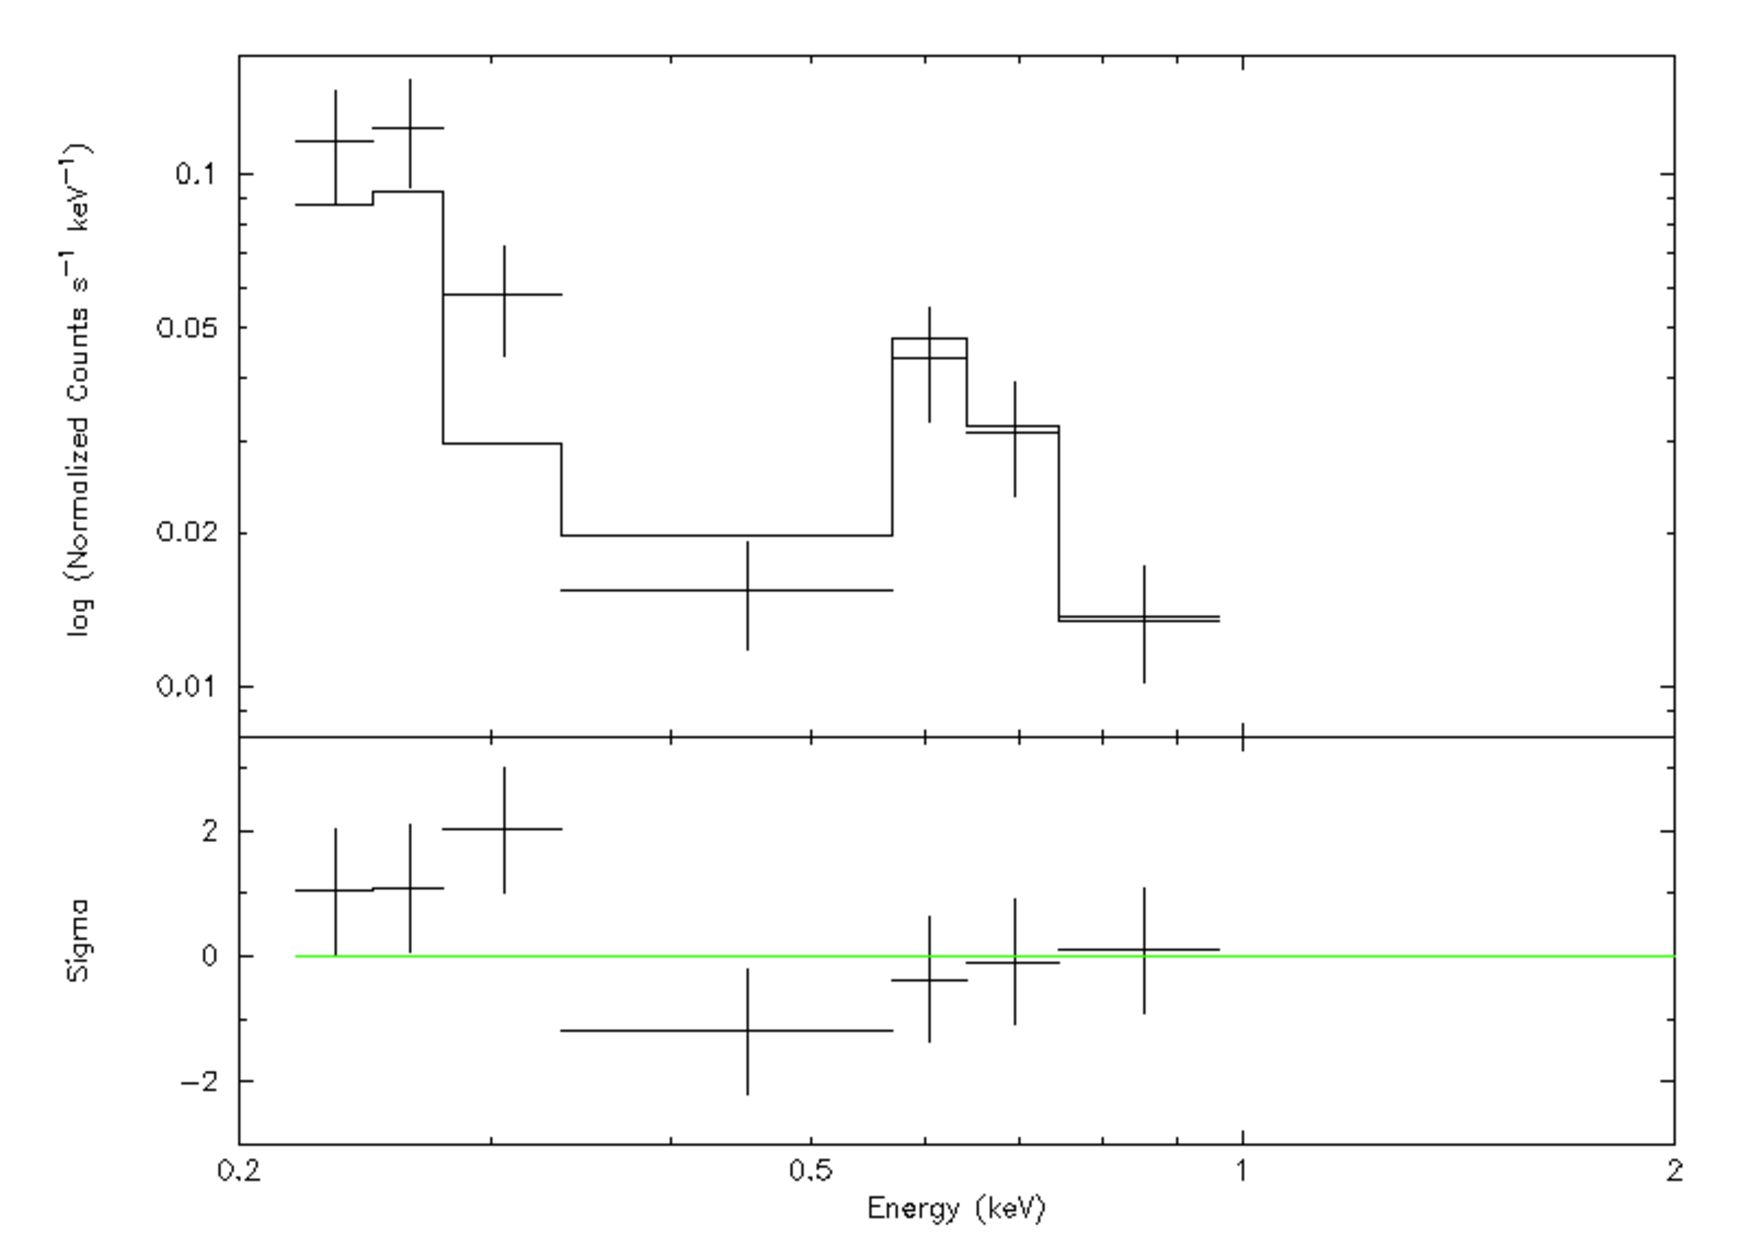
\includegraphics[height = 0.23\paperheight,width=0.9\textwidth]{Figures/3-Xray_age/spec_40eria}
	\caption{40 Eri A}
\end{subfigure}
\begin{subfigure}{\textwidth}
	\centering
	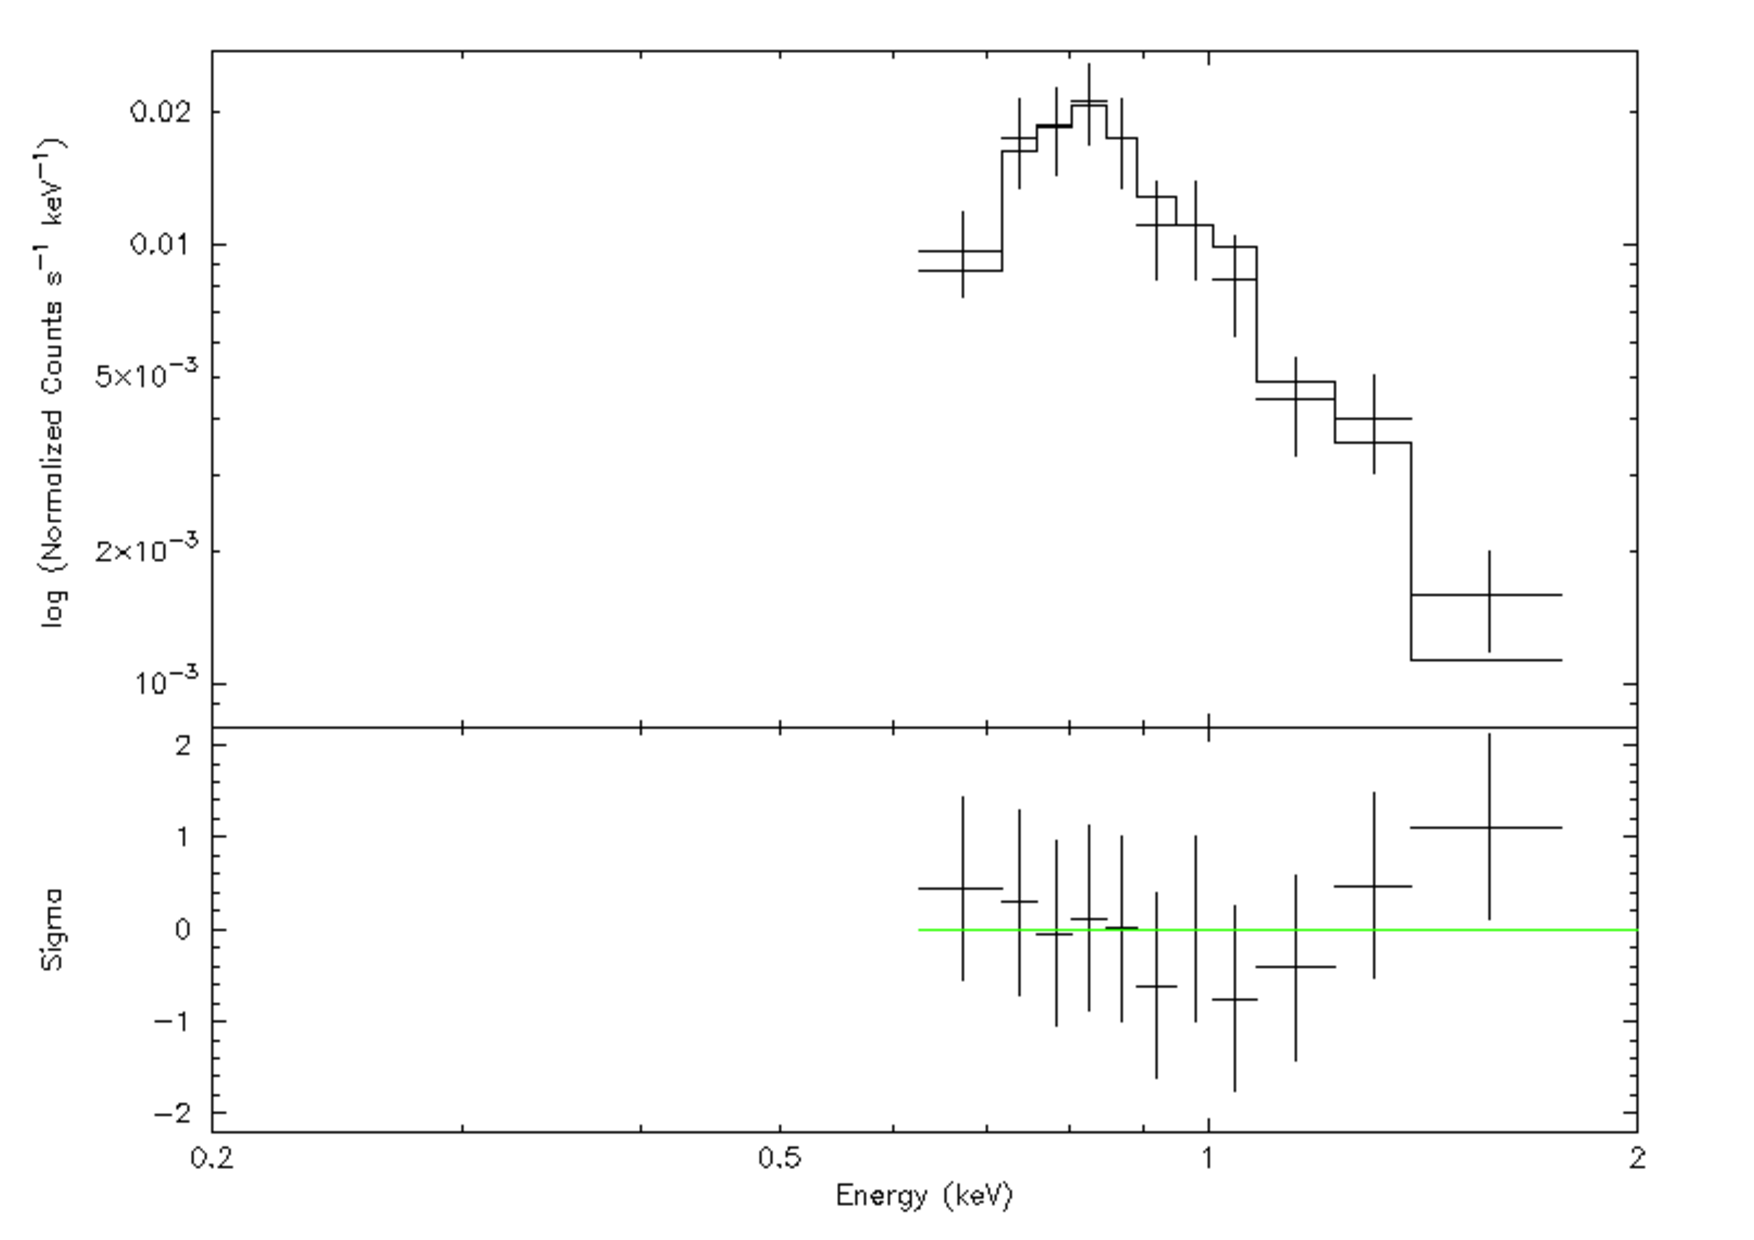
\includegraphics[height = 0.23\paperheight,width=0.9\textwidth]{Figures/3-Xray_age/spec_cd-3710500}
	\caption{CD -3710500}
\end{subfigure}

\caption[X-ray spectra of 40 Eri A and CD -3710500]{X-ray spectra (grouped to 15 counts per bin) and best fit models of two X-ray sources. The top region of each subplot shows the number of counts per second per keV as a function of energy. The bottom region of each subplot shows the sigma value for the best fit model as a function of energy. CD -3710500 was observed with a front-illuminated \textit{Chandra} CCD and therefore only has spectral data above 0.6 keV.}
\label{App_A_40EriA_CD3710500}
\end{figure}

%Second Figure
\begin{figure*}
\begin{subfigure}{\textwidth}
	\centering
	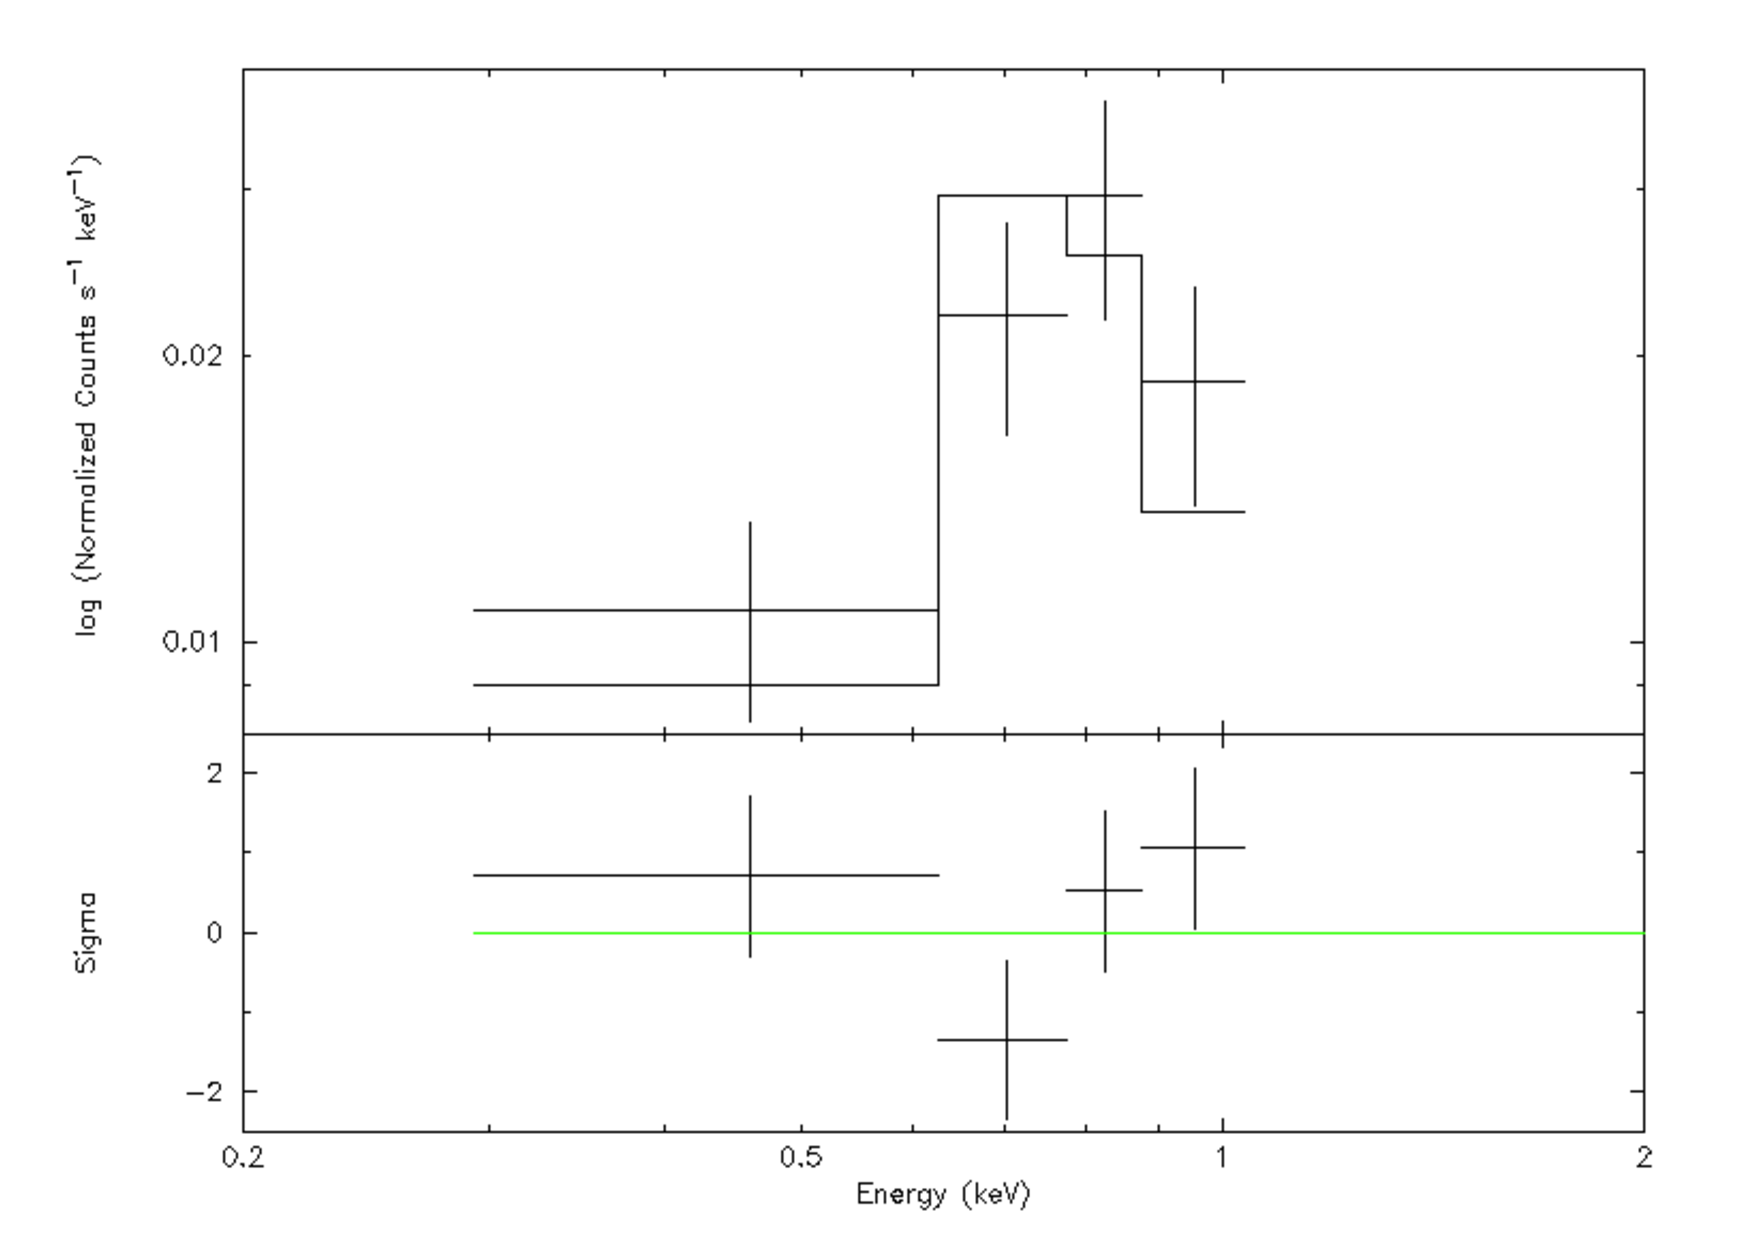
\includegraphics[height = 0.25\paperheight,width=\textwidth]{Figures/3-Xray_age/spec_gj176}
	\caption{GJ 176}
\end{subfigure}
\begin{subfigure}{\textwidth}
	\centering
	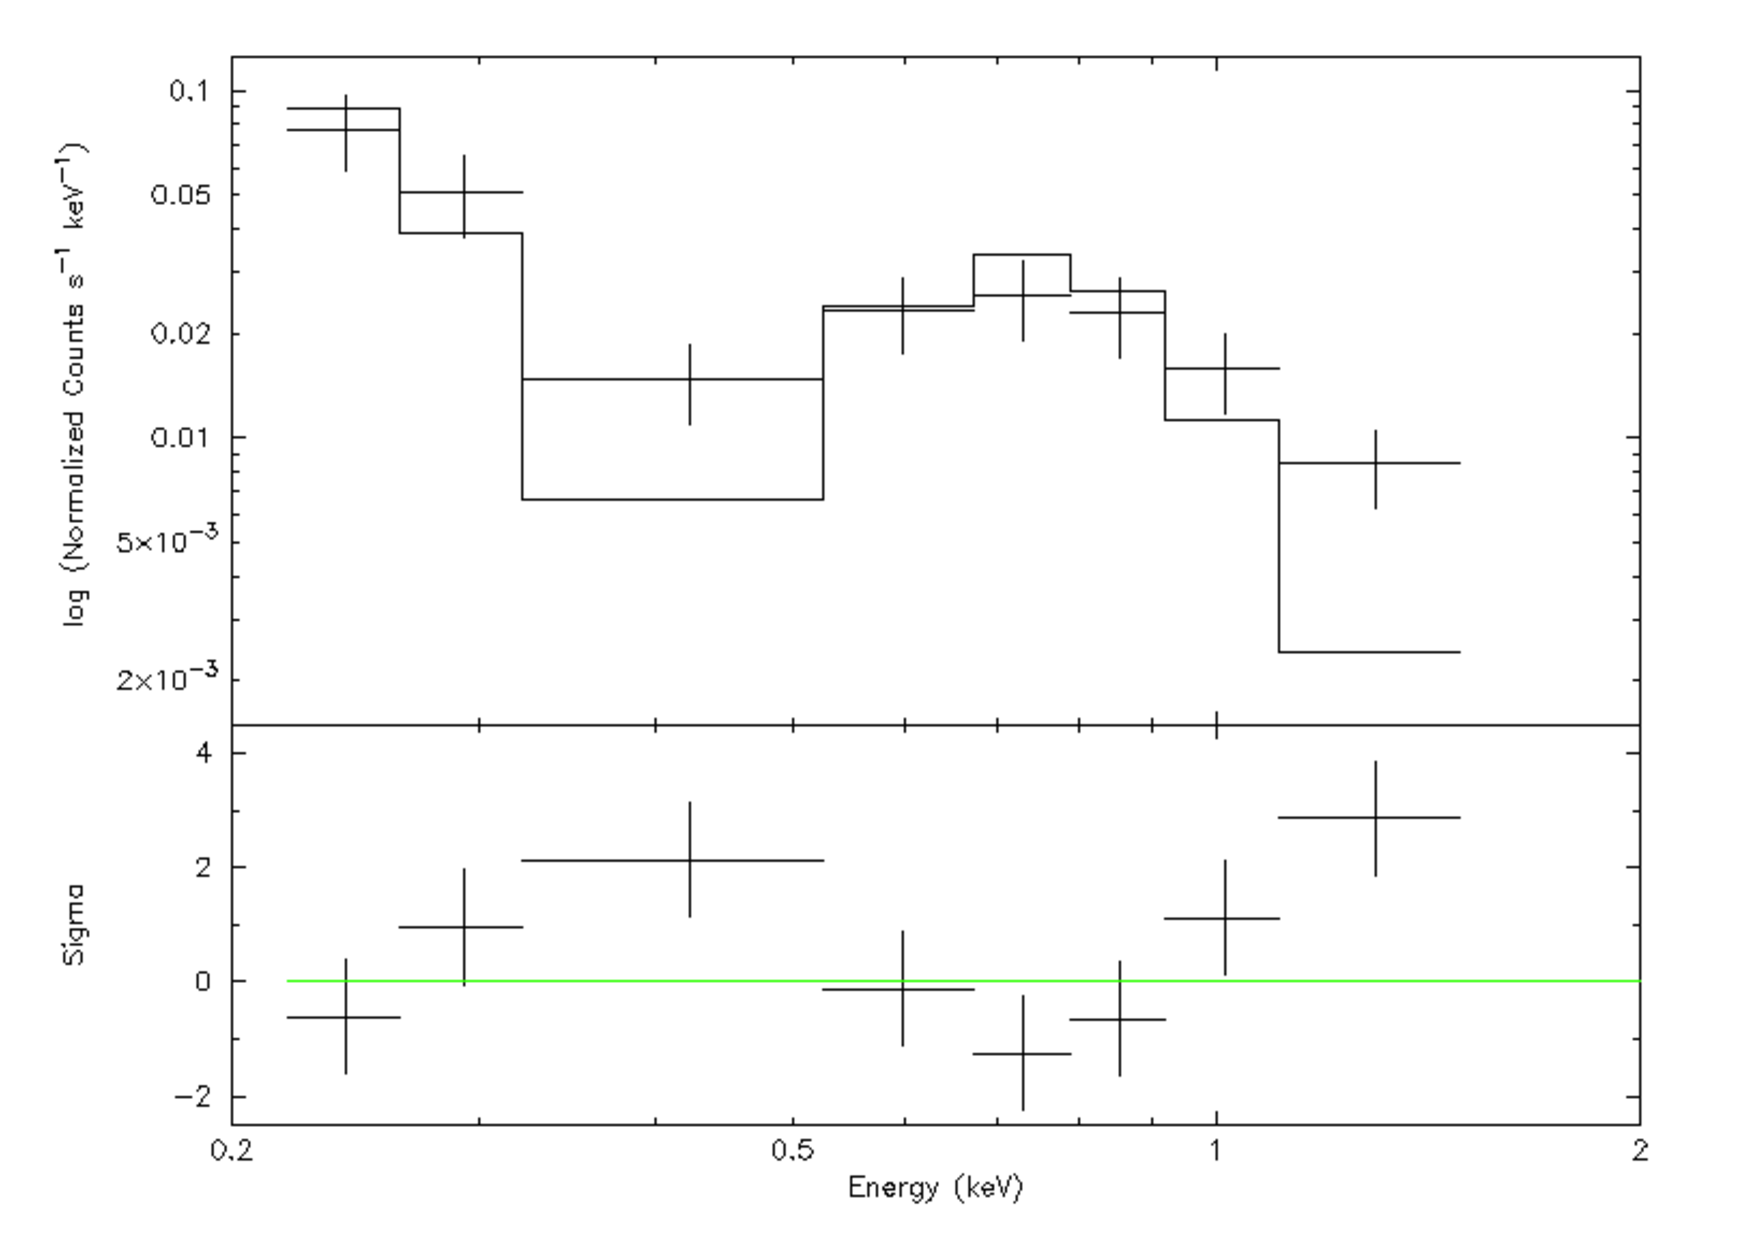
\includegraphics[height = 0.25\paperheight,width=\textwidth]{Figures/3-Xray_age/spec_gj191}
	\caption{GJ 191}
\end{subfigure}

\caption[X-ray spectra of GJ 176 and GJ 191]{X-ray spectra (grouped to 15 counts per bin) and best fit models of two X-ray sources. The top region of each subplot shows the number of counts per second per keV as a function of energy. The bottom region of each subplot shows the sigma value for the best fit model as a function of energy.}
\label{App_A_GJ176_GJ191}
\end{figure*}


%Third Figure
\begin{figure*}
\begin{subfigure}{\textwidth}
	\centering
	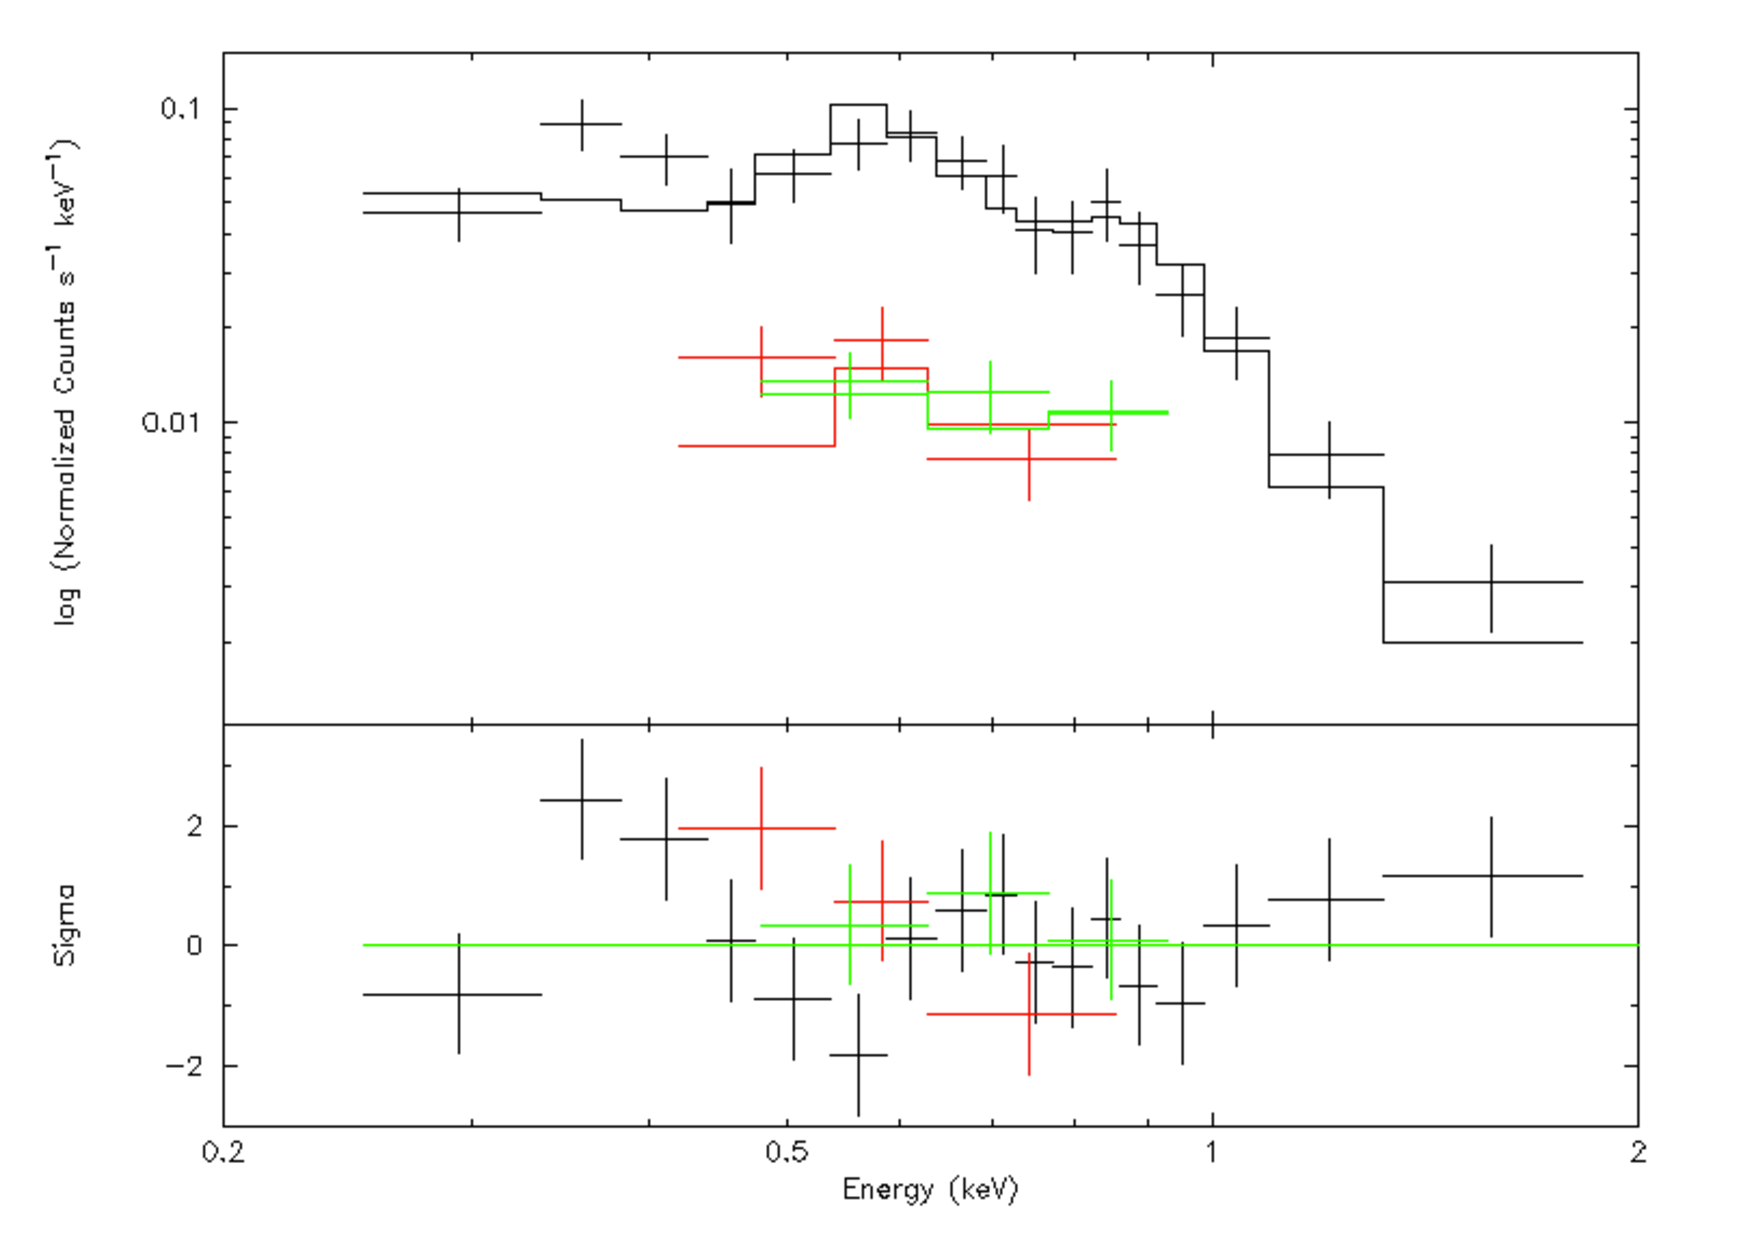
\includegraphics[height = 0.25\paperheight,width=\textwidth]{Figures/3-Xray_age/spec_hr7703}
	\caption{HR 7703}
\end{subfigure}
\begin{subfigure}{\textwidth}
	\centering
	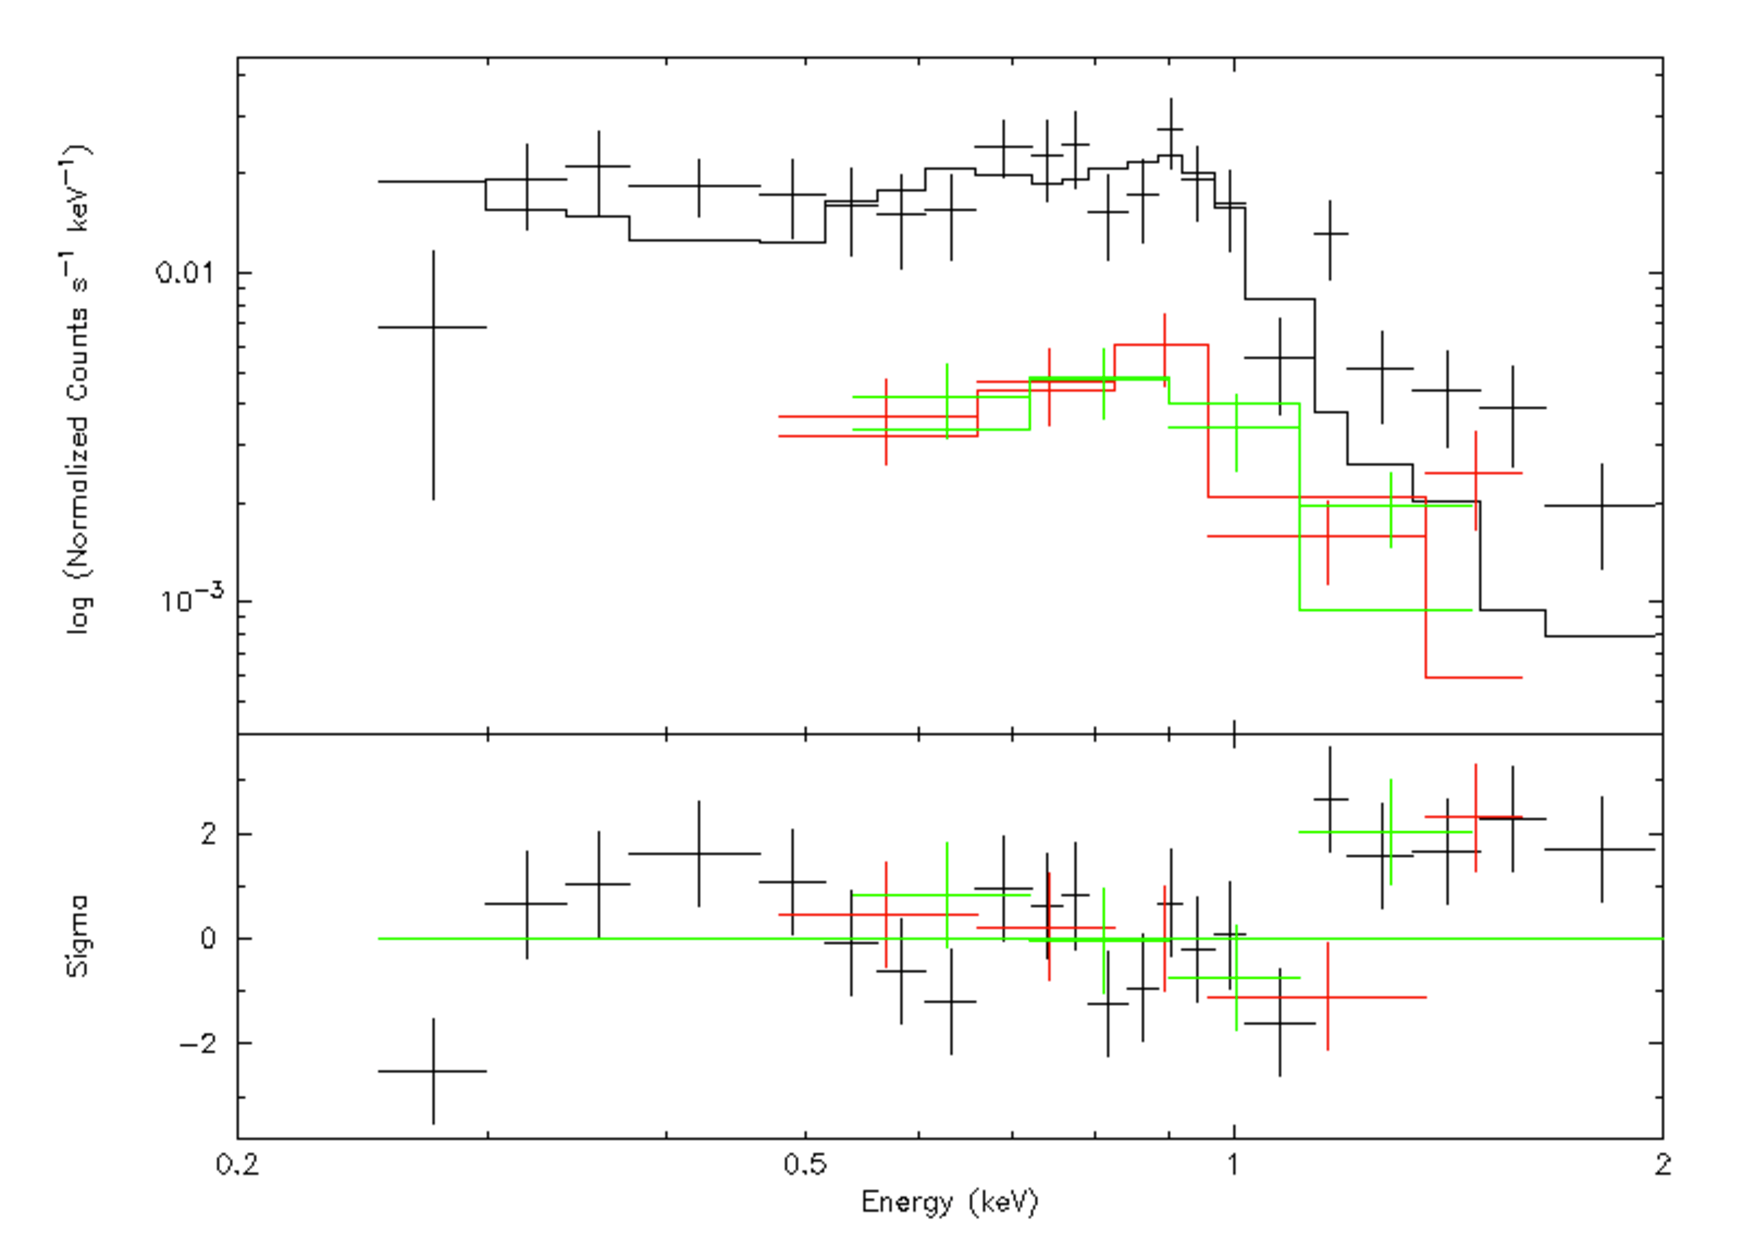
\includegraphics[height = 0.25\paperheight,width=\textwidth]{Figures/3-Xray_age/spec_kic7529180}
	\caption{KIC 7529180}
\end{subfigure}

\caption[X-ray spectra of HR 7703 and KIC 7529180]{X-ray spectra (grouped to 15 counts per bin) and best fit models of two X-ray sources. The top region of each subplot shows the number of counts per second per keV as a function of energy. The bottom region of each subplot shows the sigma value for the best fit model as a function of energy. Different colours indicate spectra from different detectors which are fitted simultaneously to ensure a more accurate fit.}
\label{App_A_HR7703_KIC7529180}
\end{figure*}

%Fourth Figure
\begin{figure*}
\begin{subfigure}{\textwidth}
	\centering
	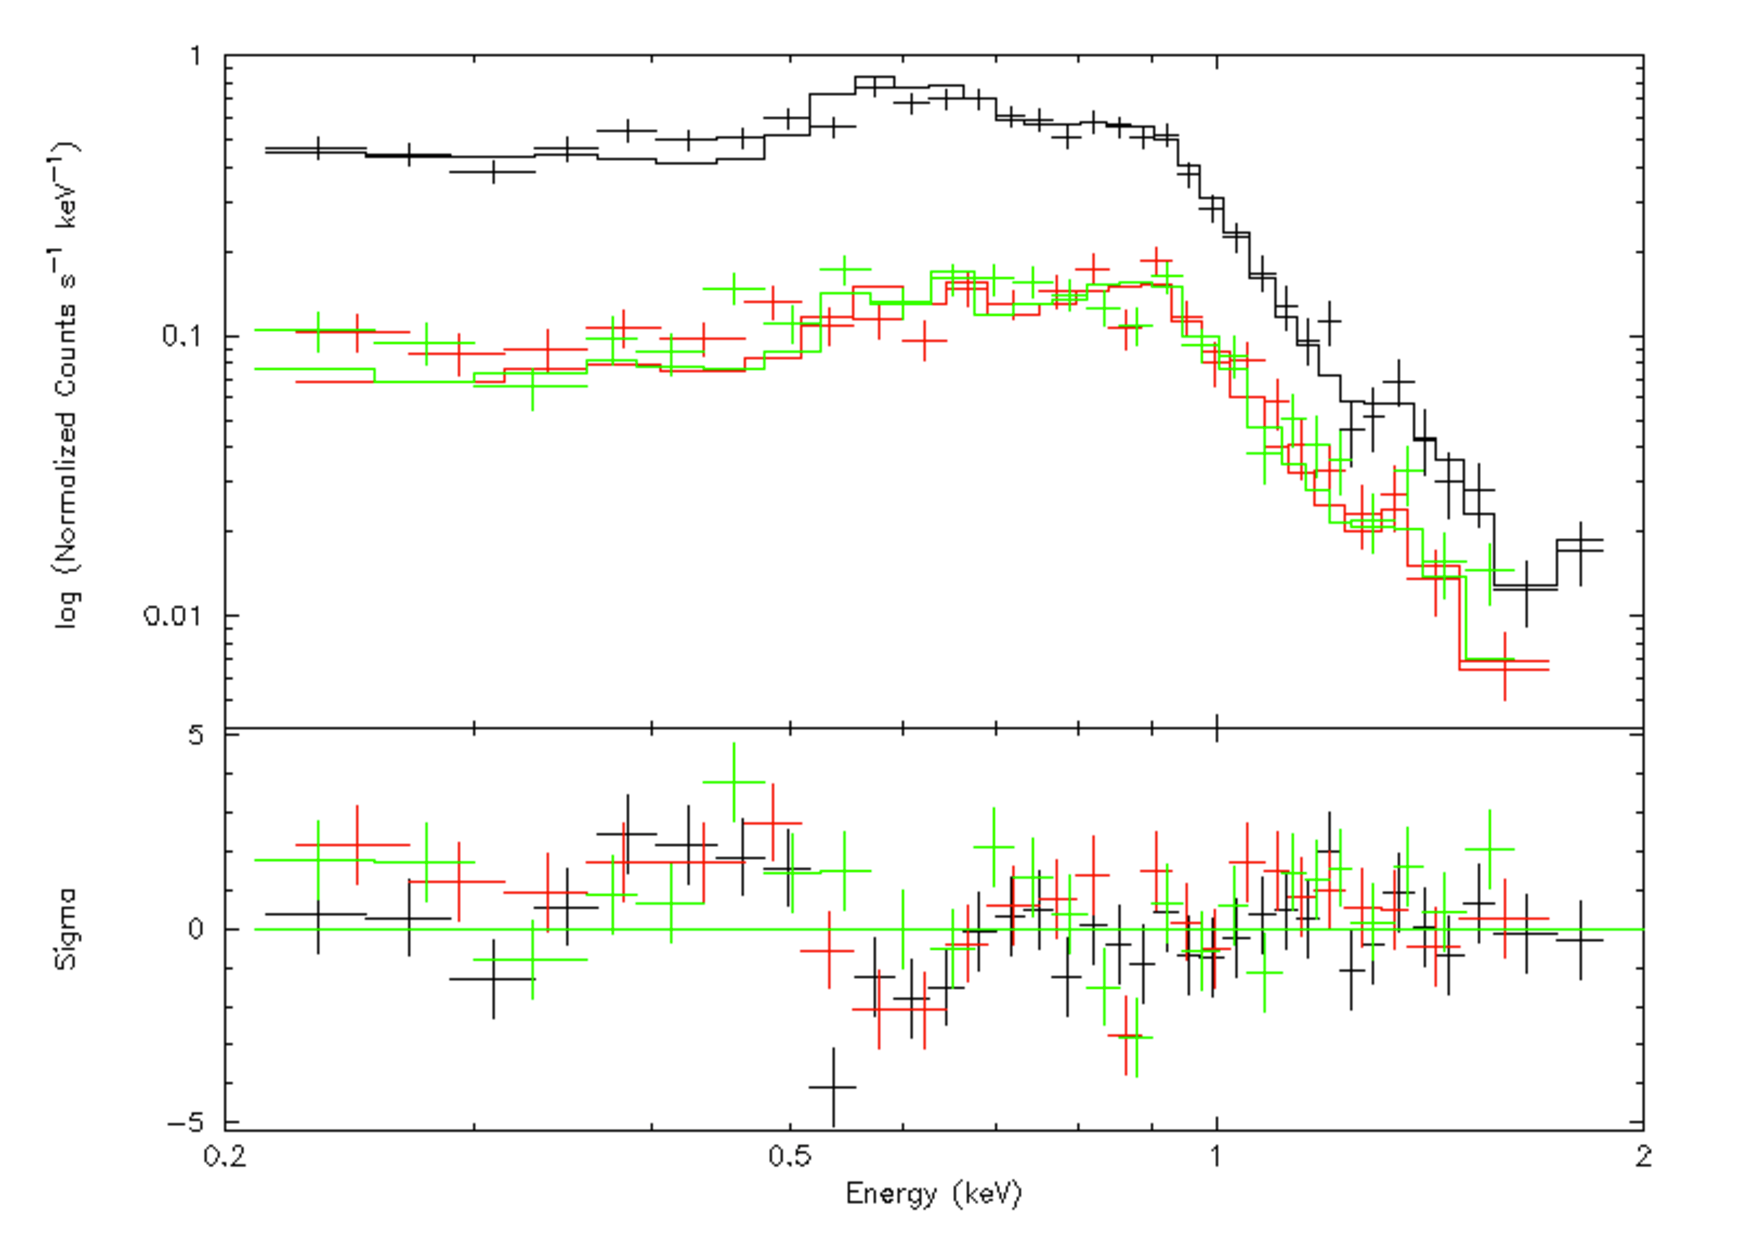
\includegraphics[height = 0.25\paperheight,width=\textwidth]{Figures/3-Xray_age/spec_61cyga}
	\caption{61 Cyg A}
\end{subfigure}
\begin{subfigure}{\textwidth}
\centering
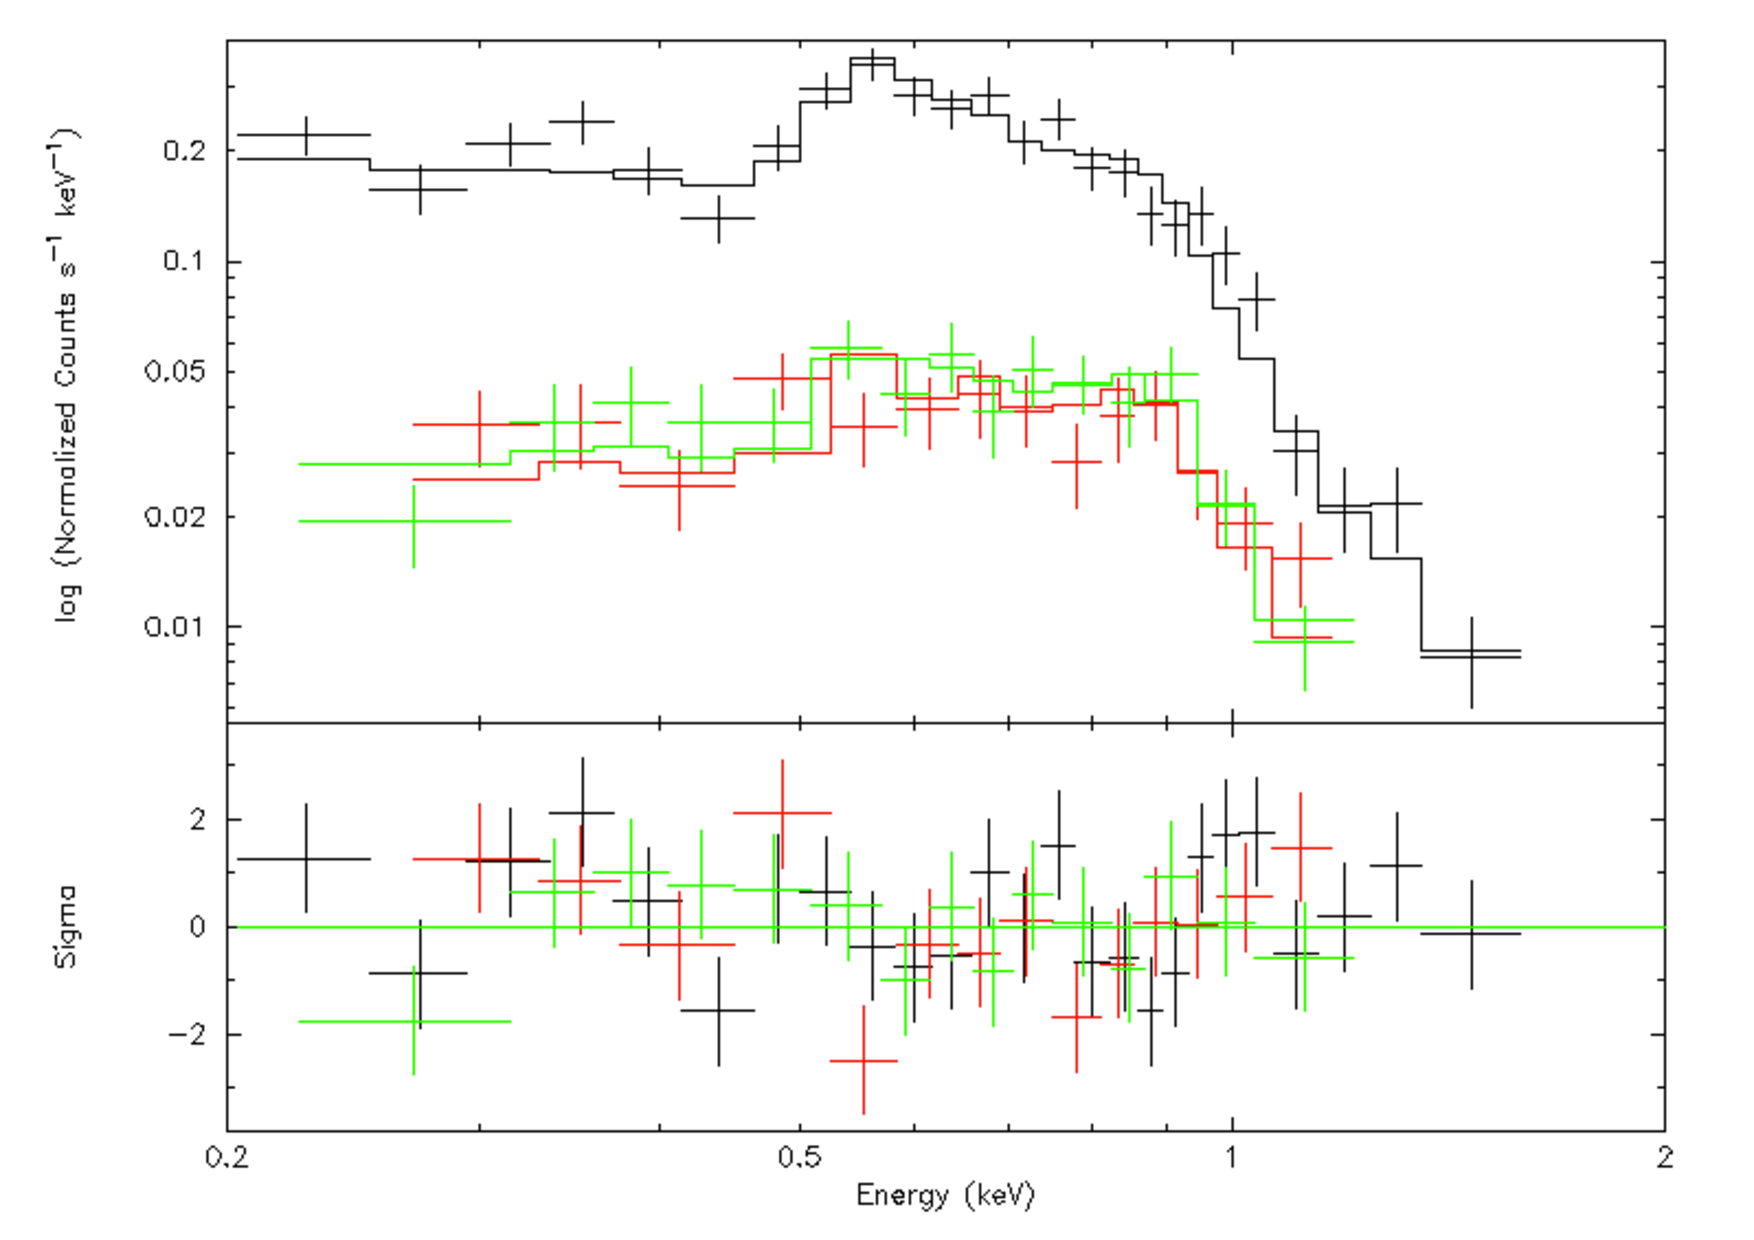
\includegraphics[height =        0.25\paperheight,width=\textwidth]{Figures/3-Xray_age/spec_61cygb}
\caption{61 Cyg B}
\end{subfigure}
\par\bigskip

\caption[X-ray spectra of 61 Cyg A and B]{X-ray spectra (grouped to 15 counts per bin) and best fit models for one exemplary observation of 61 Cyg A and B, respectively. These sources were detected to at least three sigma and contained over a hundred counts in the source region. The top region of each subplot shows the number of counts per second per keV as a function of energy. The bottom region of each subplot shows the sigma value for the best fit model as a function of energy. Different colours indicate spectra from different detectors which are fitted simultaneously to ensure a more accurate fit.}
\label{App_A_61Cyg}
\end{figure*}

%Appendix B
\chapter{X-ray luminosity and age results}
\label{App_lx_results}

\begin{table}[htbp]
    \rotatebox{90}{
    \begin{minipage}{\textheight}
		\resizebox{\textheight}{!}{
			\begin{tabular}{lccccccc}
				Name of Star / White Dwarf & Age / Gyr & log($L_{x}$ / ergs s$^{-1}$) & log($L_{x}/R_{\odot}^{2}$ / ergs s$^{-1}$ $R_{\odot}^{-2}$) & Spectral Type & Age Determination &Age Reference\\
				\hline \hline
				16 Cyg A & $6.67^{0.81}_{0.77}$  & $26.89^{0.10}_{0.10}$ & $26.71^{0.10}_{0.10}$ & G1.5Vb & Asteroseismology & 1  \\
				16 Cyg B & $7.39^{0.89}_{0.91}$ & $<25.85$   & $<25.77$ & G3V & Asteroseismology  & 1  \\
				40 Eri A / 40 Eri B & $3.70^{3.57}_{1.34}$ & $26.81^{0.10}_{0.10}$ & $26.97^{0.10}_{0.10}$ & K0.5V & White Dwarf & 4 \\
				61 Cyg A \footnote{X-ray luminosity adopted from \citet{Robrade_etal_2012}} & $6.00^{1.00}_{1.00}$ & $27.08^{0.23}_{0.23}$ & $27.43^{0.23}_{0.23}$ & K5Ve & Isochrone Fitting & 5 \\
				61 Cyg B \footnote{X-ray luminosity adopted from \citet{Robrade_etal_2012}} & $6.00^{1.00}_{1.00}$ & $26.88^{0.10}_{0.10}$ & $27.33^{0.10}_{0.10}$ & K7V & Isochrone Fitting & 5 \\
				CD -3710500 / L481-60 & $1.77^{0.65}_{0.27}$ & $28.18^{0.10}_{0.10}$ & $28.22^{0.10}_{0.10}$ & G7IV & White Dwarf & 4 \\
				GJ 176 & $2.00^{0.80}_{0.80}$ & $27.03^{0.10}_{0.10}$ & $27.80^{0.10}_{0.10}$ & M2.5V & Member of HR 1614 & 6 \\
				GJ 191 & $11.00^{1.00}_{1.00}$ & $26.41^{0.10}_{0.10}$ & $27.02^{0.10}_{0.10}$ & sdM1.0 & Galactic Halo population & 7 \\
				HR 7703 & $10.00^{2.00}_{2.00}$ & $26.80^{0.10}_{0.10}$ & $27.04^{0.10}_{0.10}$ & K2.5V & Old disk star & 8 \\
				KIC 10016239 & $2.47^{0.67}_{0.61}$ & $27.91^{0.10}_{0.10}$ & $27.71^{0.10}_{0.10}$ & F6IV & Asteroseismology & 2 \\
				KIC 12011630 & $8.48^{1.53}_{1.42}$ & $<30.06$ & $<30.05$ & G1.5V & Asteroseismology & 2 \\
				KIC 3123191 & $4.26^{0.80}_{0.75}$ & $<29.12$ & $<28.84$ & F4.5V & Asteroseismology & 2 \\
				KIC 5309966 & $3.51^{1.23}_{0.42}$ & $<29.44$ & $<29.02$ & F6V & Asteroseismology & 2 \\
				KIC 6116048 & $9.58^{2.16}_{1.90}$ & $<26.89$ & $<26.74$ & F9IV-V & Asteroseismology & 1 \\
				KIC 6603624 & $7.82^{0.94}_{0.86}$ & $<27.08$ & $<26.96$ & G8IV-V & Asteroseismology & 1 \\
				KIC 7529180 & $1.93^{0.35}_{0.30}$ & $28.98^{0.10}_{0.10}$ & $28.66^{0.10}_{0.10}$ & F5IV-V & Asteroseismology & 2 \\
				KIC 8292840 & $3.85^{0.81}_{0.75}$ & $<28.14$ & $<27.88$ & F7V & Asteroseismology & 3 \\
				KIC 9025370 & $6.55^{1.26}_{1.13}$ & $<27.24$ & $<27.23$ & F8 & Asteroseismology & 1 \\
				KIC 9410862 & $6.93^{1.49}_{1.33}$ & $<27.98$ & $<27.86$ & F7V & Asteroseismology & 1 \\
				KIC 9955598 & $6.98^{0.40}_{0.50}$ & $26.90^{0.10}_{0.10}$ & $27.01^{0.10}_{0.10}$ & K0V & Asteroseismology & 3 \\
				NLTT 7887 / NLTT 7890 & $4.97^{8.80}_{3.00}$ & $<26.92$ & $<27.13$ & K2 & White Dwarf & 4 \\
				Proxima Centauri  \footnote{X-ray luminosity taken from \citet{Fuhrmeister_etal_2011}} & $6.13^{0.55}_{0.55}$ & $26.69^{0.10}_{0.10}$ & $28.23^{0.10}_{0.10}$ & M5.5Ve & Asteroseismology & 9 \\
				Alpha Centauri B \footnote{X-ray luminosity adopted from \citet{Robrade_etal_2012}} & $6.13^{0.55}_{0.55}$ & $27.06^{0.36}_{0.36}$ & $27.19^{0.36}_{0.36}$ & K1V & Asteroseismology & 9 \\
				Sun \footnote{X-ray luminosity adapted from model values given in \citet{Peres_etal_2000}} & $4.57^{0.02}_{0.02}$ & $26.77^{0.72}_{0.72}$ & $26.77^{0.72}_{0.72}$ & G2V & Isotopic Dating & 10 \\
				\hline  
     
			\end{tabular}}
			\caption[Full X-ray luminosity results]{\begin{footnotesize}		
		\noindent \textbf{References}: (1) \citet{Silva_Aguirre_etal_2017}; (2) this work, age recalculated with BASTA algorithm \citep{Silva_Aguirre_etal_2015} using values from \citet{Chaplin_etal_2014} and  \citet{Buchhave_Latham_2015}; (3) \citet{Silva_Aguirre_etal_2015}; (4) this work, see Section \ref{Section_sample_selection}; (5) \citet{Kervella_etal_2008}; (6) \citet{Feltzing_Holmberg_2000}; (7) \citet{Anglada_Escude_etal_2014}; (8) \citet{DeWarf_etal_2010}; (9) \citet{Miglio_Montalban_2005}; (10) \citet{Bahcall_etal_1995}
		
        \end{footnotesize}}
        
	\end{minipage}}
\end{table}

%Appendix C
\chapter{Stellar properties of X-ray sample}
\label{App_Xray_sample_stellar_properties}

\begin{table}[h]
\begin{minipage}{\textwidth}
\resizebox{\textwidth}{!}{
	\begin{tabular}[h]{l l l l l l}
		\hline \hline
		Name of Star / White Dwarf & Radius / $R_{\odot}$ & $T_{eff}$ / K & $V_{mag}$ & Distance / pc & References\\
		\hline 
		16 Cyg A & 1.22 & 5825 & 5.95 & 21.29 & 1,6,8,10 \\
		16 Cyg B & 1.10 & 5720 & 6.20 & 21.22 & 1,6,8,10  \\
		40 Eri A / 40 Eri B & 0.83  & 5225 & 4.43 & 4.98 & 5,6,8,9 \\
		61 Cyg A & 0.67 & 4450 & 5.21 & 3.49 & 4,6,8,9 \\
		61 Cyg B & 0.60 & 4050 & 6.03 & 3.50 & 4,6,8,9 \\
		CD -3710500 / L481-60 & 0.96 & 5530 & 6.01 & 15.25 & 5,6,8,10 \\
		GJ 176 & 0.41 & 3475 & 9.95 & 9.27 & 5,6,8,9 \\
		GJ 191  & 0.49 & 3680 & 8.85 & 3.91 & 5,6,8,9 \\
		HR 7703 & 0.77 & 4940 & 5.32 & 6.02 & 5,6,8,9 \\
		KIC 10016239 & 1.26 & 6482 & 9.81 & 175.93 & 3,7,8,10 \\
		KIC 12011630 & 1.01 & 5817 & 10.27 & 114.40 & 3,7,8,11 \\
		KIC 3123191 & 1.37 & 6568 & 9.90 & 167.67 & 3,7,8,10 \\
		KIC 5309966 & 1.62 & 6356 & 10.62 & 288.60 & 3,7,8,10 \\
		KIC 6116048 & 1.19 & 6072 & 8.47 & 75.15 & 1,7,8,10 \\
		KIC 6603624 & 1.15 & 5612 & 9.19 & 83.56 & 1,7,8,10 \\
		KIC 7529180 & 1.45 & 6682 & 8.49 & 108.53 & 3,7,8,10 \\
		KIC 8292840 & 1.35 & 6239 & 10.51 & 250.69 & 2,2,8,9 \\
		KIC 9025370 & 1.00 & 5659 & 8.95 & 87.42 & 1,7,8,10 \\
		KIC 9410862 & 1.16 & 6230 & 10.78 & 202.27 & 1,7,8,10 \\
		KIC 9955598 & 0.88 & 5434 & 9.64 & 69.39 & 2,7,8,10 \\
		NLTT 7887 / NLTT 7890 & 0.78 & 5040 & 9.84 & 41.16 & 5,6,8,10 \\
		Proxima Centauri & 0.17 & 2925 & 11.13 & 1.30 & 5,6,8,9 \\
		Alpha Centauri B & 0.86 & 5316 & 1.33 & 1.35 & 12,12,8,12 \\
		Sun  & 1.00 & 5777 & -26.74 & 1 AU & 13 \\    
		\hline 
	\end{tabular}}
	
	\caption[Stellar properties of X-ray luminosity sample]{\begin{footnotesize}		
	\noindent
	\textbf{References}: (1) \citet{Silva_Aguirre_etal_2017}; (2) \citet{Silva_Aguirre_etal_2015}; (3) this work, radius recalculated with BASTA algorithm \citep{Silva_Aguirre_etal_2015} using values from \citet{Chaplin_etal_2014} and  \citet{Buchhave_Latham_2015}; (4) \citet{Kervella_etal_2008}; (5) Radius calculated from $T_{eff}$ and absolute brightness; (6) $T_{eff}$ estimated from Spectral Type using Table 5 from \citet{Pecaut_Mamajek_2013}; (7) \citet{Chaplin_etal_2014}
	(8) $V_{mag}$ from SIMBAD; (9) Parallax from SIMBAD; (10) Parallax from \textit{Gaia} DR1 \citep{Gaia_Collaboration_2016_DR1}; (11) Distance from Barnes-Evans method (see Section \ref{Section_Xray_distances_and_spectype} for details); (12) \citet{DeWarf_etal_2010}
	\end{footnotesize}}
	
	

\end{minipage}
\end{table}


















\end{appendices}